\documentclass[skript.tex]{subfiles}

\begin{document}
	\chapter{$\boldsymbol{L^p}$-Räume}
	\setcounter{cntr}{0}
		
	\begin{notat*}
		Im Folgenden sei $(X,\Sigma,\mu)$ ein Maßraum.
	\end{notat*}

	\begin{defin}[$L^p$-„Norm“]
		Die \emph{$L^p$-Norm} einer messbaren Funktion $f \colon (X,\Sigma) \to (\mbb{R},\mc{B})$ wird durch
		\[
			\lVert f \rVert_{L^p} \coloneqq \left(
				\int_X |f|^p \md \mu
			\right)^{\nicefrac{1}{p}}, \quad p \in [1,\infty)
		\]
		erklärt.
		\medskip\\
		Mit $\ms{L}^p(X,\mu)$ bezeichnen wir die Menge aller messbaren Funktionen $f \colon (X,\Sigma) \to (\mbb{R},\mc{B})$, deren $L^p$-Norm endlich ist.\\
		Zunächst ist $\ms{L}^p(X,\mu)$ wegen
		\[
			|f+g|^p \leq 2^p \max(|f|,|g|)^p \leq 2^p(|f|^p+|g|^p)
		\]
		ein Vektorraum.
	\end{defin}
	\paragraph{Ziele:}
	\begin{enumerate}[(1)]
		\item $L^p$-Norm ist tatsächlich eine Norm. (Problem: Nullmengen -- herausteilen $\rightarrow L^p$-Raum)
		\item Dreiecksungleichung mit Minkowski ($\impliedby$ Hölder $\impliedby$ Jensen)
		\item $L^p$-Räume sind Banachräume
		\item Approximation von $L^p$-Funktionen
	\end{enumerate}

	\begin{lem}
		Sei $f \colon (X,\Sigma) \to (\mbb{R},\mc{B})$ messbar.\\
		Dann gilt
		\[
			\int_X |f|^p \md \mu = 0 \iff f=0 \text{\quad$\mu$-fast überall.}
		\]
	\end{lem}
	\begin{proof}
		Mit $g \coloneqq |f|^p$ erhalten wir aus \emph{Lemma I.52}
		\[
			\int_X g \md\mu = 0 \iff g=0 \text{\quad$\mu$-f.\,ü.} \iff f=0 \text{\quad$\mu$-f.\,ü.}
		\]
	\end{proof}

	Also folgt $\lVert g \rVert_{L^p} = 0 \implies g = 0$ $\mu$-fast überall.\\
	Wir setzen
	\[
		\mc{N}(X,\mu) = \{f \colon (X,\Sigma) \to (\mbb{R},\mc{B}) \mid f \text{ messbar, } f(x)=0 \text{ $\mu$-f.\,ü.} \}.
	\]
	Offenbar ist $\mc{N}$ ein linearer Unterraum von $\ms{L}^p$. Insofern können wir den Quotientenraum\footnote{
		Sei $V$ ein Vektorraum und $U \subset V$ ein Unterraum.
		Für $v_1, v_2 \in V$ wird durch $v_1 \sim v_2 :\Longleftrightarrow v_1-v_2 \in U$ eine Äquivalenzrelation definiert.
		Es ist also für jeden Punkt $v \in V$ die Äquivalenzklasse \\$[v] \coloneqq v+U \coloneqq \{v+u \mid v \in U \}$. 
		Der Quotienten- bzw. Faktorraum von $V$ nach $U$ ist durch \\$V/U \coloneqq \{[v] \mid v \in V\}$ definiert.} bilden und definieren
	\[
		L^p(X,\mu) \coloneqq \ms{L}^p(X,\mu) / \mc{N}(X,\mu).
	\]
	Für $X \subset \mbb{R}^n$ schreiben wir $L^p(X) \coloneqq L^p(X,\lambda^n)$.\\
	Aus \emph{Lemma 2} folgt die Wohldefiniertheit der $L^p$-Norm auf $L^p$.\\ Man beachte, dass für $f \in L^p(X,\mu)$ und $x \in X$ der Wert $f(x)$ im Allgemeinen nicht wohldefiniert ist (es sei denn, es gibt einen stetigen Vertreter von $f$ und stetige Funktionen mit unterschiedlichen Werten gehören zu verschiedenen Äquivalenzklassen in $L^p$, z.\,B. $\lambda^n$).\medskip\\
	Im Fall $p=2$ haben wir einen Hilbertraum (d.\,h. einen vollständigen (wegen Riesz-Fischer) normierten Raum mit Skalarprodukt $\langle f,g\rangle = \int_X f(x) \overline{g(x)} \md \mu(x)$). \\
	Im Fall $p=\infty$ definieren wir das \emph{essentielle Supremum} von $f$
	\begin{align*}
		\lVert f \rVert_{L^\infty} &\ceq \inf\{s \geq 0 \mid \mu(\{x \in X \mid |f(x)| \geq s \}) = 0 \} \\
		&= \sup\{s \geq 0 \mid \mu(\{x \in X \mid |f(x)| \geq s \}) > 0 \}
	\end{align*}
	Wir bezeichnen mit $B(X,\mu)$ die Menge der essentiell beschränkten Funktionen und wir setzen wie gehabt
	\[
	L^\infty(X,\mu) = B(X,\mu) / \mc{N}(X,\mu)
	\]
	und $\lVert f \rVert_{L^\infty(x,\mu)}$ ist nach Konstruktion unabhängig vom gewählten Vertreter.
	\begin{bsp}
		\[
			\lVert \rchi_\mbb{Q} \rVert_{L^\infty(\mbb{R},\lambda)} = 0, \quad
			\lVert \rchi_\mbb{Q} \rVert_{L^\infty(\mbb{R},\underset{\displaystyle\mathclap{\overset{\uparrow}{\text{Dirac}}}}{\delta_0})} = 1
 		\]
	\end{bsp}
	Sei $X$ ein metrischer Raum, der \emph{lokalkompakt} ist (d.\,h. jeder Punkt aus $X$ besitzt eine kompakte Umgebung).\\
	Dann heißt $f \colon (X,\Sigma) \to (\mbb{R},\mc{B})$ \emph{lokal $p$-integrierbar}, falls $f \in L^p(K,\mu)$ für jedes Kompaktum $K \sbs X$ gilt. \\
	Die Menge aller lokal $p$-integrierbaren Funktionen (bzw. die Menge deren Äquivalenzklassen) wir mit $L_\text{loc}^p(X,\mu)$ bezeichnet.
	
	\section{Ungleichungen}
	\paragraph{Erinnerung:} Eine reelle Funktion $\phi\colon(a,b)\to(\mbb{R})$ heißt \emph{konvex}, falls
	\[
		\phi(\lambda x + (1-\lambda)y) \leq \lambda \phi(x) + (1-\lambda) \phi(y)
	\]
	für alle $x,y \in (a,b)$, $\lambda\in(0,1)$ bzw. \emph{strikt konvex}, wenn die strikte Ungleichung (also „$<$“) gilt.
	\begin{center}
	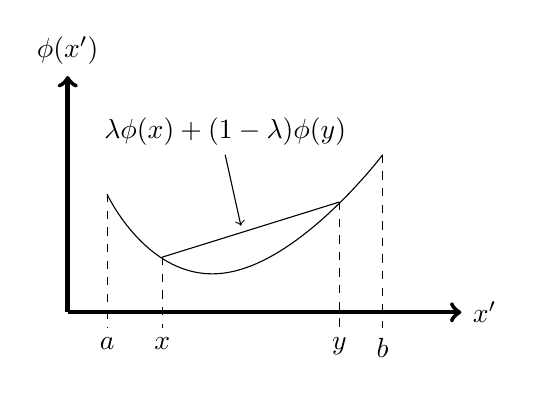
\begin{tikzpicture}
		\draw[->,ultra thick] (0,0)--(5,0) node[right]{$x'$};
		\draw[->,ultra thick] (0,0)--(0,3) node[above]{$\phi(x')$};
		
		\draw plot[smooth, tension=1] coordinates{(.5,1.5) (2,.5) (4,2)};
		\draw[dashed] (.5,1.5)--(.5,-.2) node[below]{$a$};
		\draw[dashed] (4,2)--(4,-.2) node[below]{$b$};
		
		\draw (1.2,.7)--(3.45,1.4);
		\draw[dashed] (1.2,.7)--(1.2,-.2) node[below]{$x$};
		\draw[dashed] (3.45,1.4)--(3.45,-.2) node[below]{$y$};
		
		\draw[<-] (2.2,1.1)--(2,2) node[above]{$\lambda \phi(x) + (1-\lambda) \phi(y)$};
	\end{tikzpicture}
	\end{center}
	Jede Norm auf einem Vektorraum $X$ ist konvex, denn für $f,g \in X$ und $\lambda \in (0,1)$ gilt
	\[
		\lVert \lambda f+(1-\lambda)g \rVert_X \leq \lambda \lVert f \rVert_X + (1-\lambda) \lVert g \rVert_X.
	\]
	Wir erhalten für jede konvexe Funktion $\phi$ mit $a<x<z<y<b$, also $z=\lambda x+(1-\lambda)y$ für ein $\lambda\in(0,1)$
	\[
		(\ast)\quad
		\frac{\phi(z)-{\phi(x)}}{z-x}
		\leq \frac{\phi(y)-{\phi(x)}}{y-x}
		\leq \frac{\phi(y)-{\phi(z)}}{y-z}
	\]
	und die Ungleichung ist strikt, wenn $\phi$ strikt konvex ist.
	
	\begin{lem}
		Die folgenden Aussagen gelten für jedes konvexe $\phi \colon (a,b) \to \mbb{R}$:
		\begin{enumerate}[(i)]
			\item Die Funktion $\phi$ ist lokal Lipschitz-stetig, d.\,h. für jedes kompakte Intervall $I\sbs(a,b)$ gibt es ein $L_I < \infty$ mit $|\phi(x)-\phi(y)| \leq L_I |x-y|$ für alle $x,y \in I$.
			\item Die links- und rechtsseitigen Ableitungen
			\[
				\phi'_\pm(x) = \lim_{h \searrow 0} \frac{\phi(x\pm h)-\phi(x)}{\pm h}
			\]
			existieren und sind monoton nicht-fallend.\\
			Darüber hinaus existiert $\phi'$ bis auf eine Nullmenge.
			\item Für ein festes $\bar{x} \in (a,b)$ und jedes $\alpha \in [\phi'_-(\bar{x}),\phi'_+(x)]$ gilt
			\[
				\phi(y) \geq \phi(\bar{x}) + \alpha (y-\bar{x}) \quad\forall y \in (a,b).
			\]
			Diese Ungleichung ist strikt für strikt konvexe $\phi$ und $y \neq \bar{x}$.
		\end{enumerate}
	\end{lem}
	\begin{proof}
		Setze $D(x,y) \ceq \frac{\phi(x)-\phi(y)}{x-y}$. Aus $(\ast)$ folgt
		\[
			D(x,z) \leq D(x,y) \leq D(y,z)
		\]
		für $x<z<y$.\\
		Damit ist $0 < \epsilon_1 < \epsilon_2 \implies D(\underbrace{x+\epsilon_1}_{=z},x) \leq D(\underbrace{x+\epsilon_2}_{=y},x)$, also $\epsilon \mapsto D(x+\epsilon,x)$ monoton steigend und (auf Kompakta) beschränkt. Folglich existiert $\phi'_+(x)$ und analog $\phi'_-(x)$.\\
		Wegen $D(x-\epsilon,x) \leq D(x+\epsilon,x)$ folgt $\phi'_-(x) \leq \phi'_+(x)$ und weiter $\phi'_+(x) \leq \phi'_-(y)$ für $x<y$, sodass wir insgesamt
		\[
			\phi'_-(x) \leq \phi'_+(x) \leq \phi'_-(y) \leq \phi'_+(y)
		\]
		erhalten.\\
		Da eine monotone Funktion nur abzählbar viele Sprungstellen haben kann, folgt \emph{(ii)}.\\
		Aus $(\ast)$ gewinnen wir direkt $\phi'_+(x) \leq D(x,y) \leq \phi'_-(y)$, was die äquivalenten Ungleichungen
		\[
			\phi(y) \geq \phi(x) + \phi'_\pm(x)(y-x)
			\iff \phi(y) \geq \phi(x) + \alpha(y-x)
		\]
		impliziert $\Rightarrow$ \emph{(iii)}.\\
		
		Für $a<\alpha<x<y<\beta<b$ ist
		\[
			\phi'_+(\alpha) \leq D(x,y) \leq \phi'_-(\beta).
		\]
		Somit folgt \emph{(i)} mit $L_{[\alpha,\beta]} \ceq\{\abs{\phi'_+(\alpha)},\abs{\phi'_-(\beta)}\}$.
	\end{proof}

	\begin{theorem}[Jensen]
		Sei $\phi \colon (a,b) \to \mbb{R}$ konvex für $-\infty \leq a<b \leq +\infty$.\\
		Ist $\mu$ ein Wahrscheinlichkeitsmaß auf $(X,\Sigma)$ und $f \in \ms{L}^1(X,\mu)$ mit $a<f(x)<b$ für alle $x \in X$, dann ist der negative Teil von $\phi \circ f$ integrierbar und
		\[
			\phi\left(\int_X f \md\mu\right) \leq \int_X (\phi \circ f) \md\mu.
		\]
		Ist $\phi \geq 0$ nicht-fallend, $f \geq 0$ und $\phi(b) \ceq \lim_{x \nearrow b} \phi(x)$, so gilt die Schlussfolgerung auch für nicht-integrierbare (messbare) $f$.
	\end{theorem}
	\begin{proof}
		Eigenschaft \emph{(iii)} des Lemmas impliziert
		\[
			\phi(\underbrace{f(x)}_{\in(a,b)}) \geq
			\underbrace{\phi(\bar{x})}_{\in\mbb{R}} +
			\uarrow{\in\mbb{R}}{\alpha}(f(x)-\uarrow{\in\mbb{R}}{\bar{x}}) \quad \forall x \in X \text{ und } \bar{x} = \int_X f \md\mu \in(a,b).
		\]
		Damit ist $(\phi \circ f)_-$ integrierbar und wir erhalten
		\[
			\int_X \phi(f(x)) \md\mu(x) \geq \phi(\bar{x}) + \alpha \left( \int_X f(x) \md\mu(x) - \bar{x} \right),
		\]
		was die Behauptung für $f \in \ms{L}^1(X,\mu)$ zeigt.\\
		Ist nun $f \geq 0$, aber $f \notin \ms{L}^1(X,\mu)$, so setzen wir $X_n \ceq \{x \in X \mid \underbrace{f(x)}_{\mathclap{\geq 0 \text{ n.\,V.}}} \leq n \}$ und erhalten aus dem bislang Gezeigten
		\[
			\phi\left(\frac{1}{\mu(X_n)} \int_{X_n} f \md\mu\right)
			\leq \frac{1}{\mu(X_n)} \int_{X_n} (\phi \circ f) \md\mu.
		\]
		Für $n \to \infty$ erhalten wir wegen $X_n \nearrow X$ einerseits $\mu(X_n) \nearrow \mu(X)$ und die Konvergenz der Integrale aus dem Satz über monotone Konvergenz.
	\end{proof}
	
\end{document}
